% BTech Project-I report, condensed edition (at most 50 pages).
% Build inside report/: tectonic final_report_50.tex
% Every number is taken from final_report.tex / phase2_chapter.tex, which cite the repository sources.
\documentclass[12pt,a4paper,oneside]{report}

\usepackage{fontspec}
\setmainfont{texgyretermes}[Extension=.otf,UprightFont=*-regular,BoldFont=*-bold,ItalicFont=*-italic,BoldItalicFont=*-bolditalic]
\setmonofont{lmmono10-regular}[Extension=.otf,Scale=0.95,BoldFont=lmmonolt10-bold,ItalicFont=lmmono10-italic,BoldItalicFont=lmmonolt10-boldoblique]
\usepackage[a4paper,left=3.5cm,right=2.5cm,top=2.5cm,bottom=2.5cm,headheight=14pt]{geometry}
\usepackage{setspace}
\onehalfspacing
\usepackage{graphicx}
\usepackage{booktabs}
\usepackage{tabularx}
\usepackage{array}
\usepackage{multirow}
\usepackage{xcolor}
\usepackage{enumitem}
\usepackage{caption}
\captionsetup{font=small,labelfont=bf}
\usepackage{tikz}
\usetikzlibrary{arrows.meta,positioning}
\usepackage{tfrupee}
\usepackage[numbers,sort&compress]{natbib}
\usepackage{titlesec}
\titleformat{\chapter}[display]{\normalfont\Large\bfseries}{\chaptertitlename\ \thechapter}{10pt}{\LARGE}
\titlespacing*{\chapter}{0pt}{-30pt}{18pt}
\usepackage{fancyhdr}
\pagestyle{fancy}
\fancyhf{}
\fancyhead[R]{\small\nouppercase{\leftmark}}
\fancyfoot[C]{\thepage}
\renewcommand{\headrulewidth}{0.4pt}
\fancypagestyle{plain}{\fancyhf{}\fancyfoot[C]{\thepage}\renewcommand{\headrulewidth}{0pt}}
\usepackage{xurl}
\usepackage[hidelinks]{hyperref}
\usepackage{seqsplit}
\usepackage{makecell}
\usepackage{float}
\let\oldunderscore\_
\renewcommand{\_}{\oldunderscore\allowbreak}
\setlength{\emergencystretch}{3em}
\newcommand{\hash}[1]{\texttt{\seqsplit{#1}}}
\newcommand{\rs}{\rupee}
\newcommand{\form}[1]{\textbf{#1}}
\newcolumntype{L}{>{\raggedright\arraybackslash}X}
\setlist{nosep}

\begin{document}

%======================================================================
% TITLE PAGE
%======================================================================
\begin{titlepage}\singlespacing
\begin{center}
\vspace*{-0.5cm}
{\LARGE\bfseries Romanized Hindi Is Harder Than Hinglish:\\[4pt] A Scoring-Aware Audit of Small LLMs on\\[4pt] Mathematical Word Problems\par}
\vspace{0.8cm}
{\large B.Tech.\ Project-I (MC 401) Report\par}
\vspace{0.3cm}
{\large submitted in partial fulfilment of the requirements for the award of the degree of\par}
\vspace{0.3cm}
{\Large\bfseries Bachelor of Technology\par}
\vspace{0.2cm}
{\large in\par}
\vspace{0.2cm}
{\large Mathematics and Computing\par}
\vspace{0.8cm}
{\large Submitted by\par}
\vspace{0.3cm}
{\large Divyansh Raj \enspace (23/MC/195)\par}
{\large Ayush Kumar Singh \enspace (23/MC/194)\par}
{\large Divyanshu Mishra \enspace (23/MC/196)\par}
\vspace{0.8cm}
{\large Under the supervision of\par}
\vspace{0.3cm}
{\large Dr.\ Dinesh Udar\par}
{\large Assistant Professor, Department of Applied Mathematics\par}
\vfill

\includegraphics[height=3cm]{figures/dtu_logo.png}\\[0.6cm]
{\large\bfseries Department of Applied Mathematics\\ Delhi Technological University\par}
{\large (Formerly Delhi College of Engineering)\\ Bawana Road, Delhi -- 110042\par}
\vspace{0.5cm}
{\large November 2026\par}
\end{center}
\end{titlepage}

\pagenumbering{roman}
\setcounter{page}{2}

%======================================================================
% CERTIFICATE
%======================================================================
\chapter*{Certificate}
\addcontentsline{toc}{chapter}{Certificate}
\thispagestyle{plain}
\markboth{Certificate}{}

I hereby certify that the project report entitled \textbf{``Romanized Hindi Is Harder Than Hinglish: A Scoring-Aware Audit of Small LLMs on Mathematical Word Problems''}, submitted by Divyansh Raj (23/MC/195), Ayush Kumar Singh (23/MC/194) and Divyanshu Mishra (23/MC/196) to the Department of Applied Mathematics, Delhi Technological University, in partial fulfilment of the requirements for the award of the degree of Bachelor of Technology, is a record of the project work carried out by the students under my supervision. To the best of my knowledge, this work has not been submitted in part or in full for any degree or diploma at this university or elsewhere.

\vspace{3cm}
\noindent
\begin{tabular}{@{}l@{\hspace{4cm}}l@{}}
Place: Delhi & \rule{5cm}{0.4pt}\\
Date: \rule{3cm}{0.4pt} & Dr.\ Dinesh Udar\\
 & Assistant Professor\\
 & Department of Applied Mathematics\\
 & Delhi Technological University\\
\end{tabular}

%======================================================================
% DECLARATION
%======================================================================
\chapter*{Candidate's Declaration}
\addcontentsline{toc}{chapter}{Candidate's Declaration}
\thispagestyle{plain}
\markboth{Candidate's Declaration}{}

We, Divyansh Raj (23/MC/195), Ayush Kumar Singh (23/MC/194) and Divyanshu Mishra (23/MC/196), students of B.Tech.\ (Mathematics and Computing), hereby declare that the project report entitled \textbf{``Romanized Hindi Is Harder Than Hinglish: A Scoring-Aware Audit of Small LLMs on Mathematical Word Problems''}, submitted to the Department of Applied Mathematics, Delhi Technological University, in partial fulfilment of the requirements for the award of the degree of Bachelor of Technology, is original and has not been submitted, in part or in full, for any other degree or diploma.

The use of AI assistants in the project is disclosed in full in Section~\ref{sec:aidisclosure}. Human reviewers made every dataset acceptance decision, and we take responsibility for the content of this report.

\vspace{3cm}
\noindent
\begin{tabular}{@{}c@{\hspace{0.6cm}}c@{\hspace{0.6cm}}c@{}}
\rule{4.4cm}{0.4pt} & \rule{4.4cm}{0.4pt} & \rule{4.4cm}{0.4pt}\\
Divyansh Raj & Ayush Kumar Singh & Divyanshu Mishra\\
(23/MC/195) & (23/MC/194) & (23/MC/196)\\
\end{tabular}

\vspace{1.5cm}
\noindent Place: Delhi\\[0.4cm]
Date: \rule{3cm}{0.4pt}

%======================================================================
% ACKNOWLEDGEMENTS
%======================================================================
\chapter*{Acknowledgements}
\addcontentsline{toc}{chapter}{Acknowledgements}
\thispagestyle{plain}
\markboth{Acknowledgements}{}

We are grateful to our supervisor, Dr.\ Dinesh Udar, Assistant Professor, Department of Applied Mathematics, Delhi Technological University, for guidance and support throughout this project.

We thank Prof.\ Ramesh Srivastava, Head of the Department of Applied Mathematics, and the faculty and staff of the department, for their support and for the facilities provided.

We thank the bilingual team members and volunteers who solved, reviewed and repaired the problem renderings, and the adjudicator who confirmed the reference answers for the original pilot. All reviewers consented to the release of the reviewed data under CC BY 4.0. In keeping with their stated preferences, reviewers are not named here; the adjudicator declined credit.

We also thank our families and friends for their encouragement. Model training and evaluation were run on Google Colab GPUs.

%======================================================================
% ABSTRACT
%======================================================================
\chapter*{Abstract}
\addcontentsline{toc}{chapter}{Abstract}
\thispagestyle{plain}
\markboth{Abstract}{}

{\setstretch{1.25}
A large number of Indian users type maths questions in Hinglish or in Hindi written with English letters. We asked a simple question: if the mathematics stays the same and only the language form changes, does a small open language model still get the answer right? Every problem in our data exists in three matched versions: English (\form{E}), Romanized Hindi (\form{R}) and Roman-script Hinglish (\form{C}). Gold answers are computed in code, new items are solved blind by two LLMs, and bilingual humans review them. Models are run unchanged on a free Colab T4 with one fixed English instruction, greedy decoding and a frozen strict scorer, and each cohort's analysis plan was committed before any output on it.

Testing on 36 excluded fixtures showed that one innocent-looking phrase in the answer-format instruction made 10/36 Qwen3-4B outputs fail strict scoring. One disclosed revision fixed this. A seven-model screen then admitted three models. On the primary 70-family Pilot-B cohort, accuracy on E/R/C was 94.3/85.7/94.3\% for Qwen3-4B, 98.6/91.4/98.6\% for Qwen3-8B and 94.3/57.1/70.0\% for Llama-3.2-3B. R was the weakest form for every model, and a separate 24-family cohort pointed the same way. The R errors were not concentrated in items with Hindi operation words.

In Phase~2 we fine-tuned Qwen3-4B with QLoRA in three matched arms (E+E, E+R, E+C) over three paired seeds and tested once on 100 untouched families. Hinglish training did not beat Romanized-Hindi training on Hinglish questions: $\Delta_C = -4.33$ points, 95\% interval $[-8.00, -0.67]$, the pre-registered \emph{Harm} label. All arms also lost about 24--26 points of English accuracy. Phase~3 repeats the comparison with the model's own solutions as targets; all nine runs are trained and frozen, and the single test evaluation is next.

\medskip
\noindent\textbf{Keywords:} Hinglish, Romanized Hindi, code-mixing, mathematical reasoning, LLM evaluation, pre-registration, QLoRA.\par}

%======================================================================
{\setstretch{1.1}
\tableofcontents
\listoffigures
\listoftables
}

%======================================================================
\chapter*{List of Abbreviations}
\addcontentsline{toc}{chapter}{List of Abbreviations}
\thispagestyle{plain}
\markboth{List of Abbreviations}{}

{\setstretch{1.1}
\begin{tabular}{@{}p{3.2cm}p{10.5cm}@{}}
\toprule
\textbf{Term} & \textbf{Meaning}\\
\midrule
\form{E}, \form{R}, \form{C} & English, Romanized Hindi and Roman-script Hinglish renderings\\
E+E, E+R, E+C & The three fine-tuning arms (second example in E, R or C)\\
D0xx & Entry in the project decision log (\texttt{docs/DECISIONS.md})\\
DEV, TRAIN, FINAL\_TEST & Phase-2 development, training and held-out test splits\\
FMT2 & The 12 excluded format-test fixture families (36 prompts)\\
LLM & Large language model\\
LoRA / QLoRA & Low-rank adaptation / quantized LoRA\\
NF4, FP16 & 4-bit NormalFloat quantization; 16-bit floating point\\
pp & Percentage points\\
SRW & Student Research Workshop (EACL)\\
T4 & NVIDIA Tesla T4 GPU (Google Colab)\\
\bottomrule
\end{tabular}\par}

\cleardoublepage
\pagenumbering{arabic}

%======================================================================
\chapter{Introduction}
\label{ch:intro}
%======================================================================

\section{Motivation}

Take a simple question: ``How many marbles does Aman have?'' A model may answer it correctly and still fail on \emph{Aman ke paas kitne kanche hain?}, even though the arithmetic has not changed at all. A very large number of people in India write Hindi in the Latin alphabet when they chat, search or send messages, and they mix in English words freely. If a maths assistant becomes less reliable when a student types in this everyday style, the loss falls on exactly the people these tools claim to serve.

The difficulty is in measuring it fairly. A drop in accuracy on a Hinglish question could come from Hindi vocabulary, from non-standard Roman spelling, from switching languages mid-sentence, from a clumsier wording, or simply from the scorer: a right answer written in an unexpected format is marked wrong. Comparing unrelated English and Hinglish questions cannot pull these apart. So we fixed the mathematics and changed only the language form.

\section{The E/R/C set-up}

Each \emph{family} in our data is one problem written three ways:
\begin{itemize}
\item \form{E}: plain English;
\item \form{R}: Hindi phrasing in Roman script, with a short allowed list of borrowings (numbers, units, established loanwords);
\item \form{C}: Roman-script Hindi that also carries English words beyond that list, i.e.\ Hinglish.
\end{itemize}
The model sees each version in a fresh context with the same English instruction, and one frozen scorer marks it. Because all three versions share the same maths and the same gold answer, a difference in correctness across E, R and C reflects how the model copes with the language form, provided the three texts really are equivalent and natural. Making sure of that is the job of the review process in Chapter~\ref{ch:method}.

\section{Research questions}

\begin{description}[leftmargin=1.2cm,style=nextline]
\item[RQ1 (Phase 1)] How does an unchanged model's correctness differ across mathematically equivalent E, R and C prompts?
\item[RQ2 (Phase 2)] Does E+C fine-tuning improve held-out C accuracy over matched E+R fine-tuning?
\item[RQ3 (Phase 2)] Do any gains transfer to unseen phrasing and spellings, and what happens to English accuracy?
\end{description}
Phase~3, now under way, asks RQ2 again with a different kind of training target.

\section{Contributions}

We are not the first to see Romanized Hindi score below Hinglish. CodeMixTax~\citep{sthanika-2026-codemix} reports the same ordering on 955 translated GSM8K questions, and \citet{peter-etal-2026-mind} show that translation and answer-extraction errors can distort multilingual maths gaps. Our work builds on both. What we add is:
\begin{enumerate}
\item \textbf{New triplets.} 370 frozen families drafted fresh (not taken from GSM8K) in natural Roman spelling, each with code-computed gold and blind dual-model verification. Every evaluated cohort was human-reviewed.
\item \textbf{A scoring-aware frozen protocol.} We found and fixed a format problem on excluded data before any real run, and screened seven models against a fixed compliance rule.
\item \textbf{Two separately reviewed, pre-registered cohorts}, never pooled, in which R is the lowest-scoring form for all three models.
\item \textbf{A negative result on a tempting explanation}: the R errors do not cluster in items containing Hindi operation words such as \emph{bhaag} and \emph{bhinn}.
\item \textbf{A reproducible pipeline}: self-contained Colab notebooks with journal and resume, checksummed exports, an independent table builder and 161 passing tests.
\item \textbf{A controlled, pre-registered fine-tuning study}, in which Hinglish training did worse than Romanized-Hindi training on Hinglish questions ($\Delta_C = -4.33$ points $[-8.00, -0.67]$, Harm).
\end{enumerate}

\section{How this report is organised}

Chapter~\ref{ch:lit} reviews related work. Chapter~\ref{ch:method} covers the data and the evaluation protocol, and Chapter~\ref{ch:system} the software. Chapter~\ref{ch:dev} reports what we learned on excluded fixtures, Chapter~\ref{ch:results} gives the Phase-1 results, Chapter~\ref{ch:phase2} the fine-tuning study and Chapter~\ref{ch:phase3} the status of Phase~3. Chapter~\ref{ch:limits} covers limitations, ethics and AI use, and Chapter~\ref{ch:conclusion} concludes. Results from excluded fixtures are always labelled as development evidence and kept apart from cohort results.

%======================================================================
\chapter{Literature Review}
\label{ch:lit}
%======================================================================

Our bibliography entries were each checked against a primary source (ACL Anthology, arXiv, DOI records or publisher pages). A bounded novelty check on 26 October 2026 looked at fifteen recent works. It was a targeted audit, not an exhaustive survey.

\section{Maths word problems across languages}

GSM8K~\citep{cobbe-etal-2021-gsm8k} is the usual English grade-school benchmark, with 7,473 training and 1,319 test problems that each have a numeric answer. MGSM~\citep{shi-etal-2023-mgsm} hand-translates 250 of its test problems into ten languages and finds that chain-of-thought reasoning carries across languages; Hindi is not among them. For Hindi there is GSM8K-Hi~\citep{kamath-etal-2025-benchmarking}, a human-corrected machine translation into Devanagari, and HAWP~\citep{sharma-etal-2022-hawp}, 2,336 Hindi arithmetic problems whose authors note wrong word senses and translation errors while building it. \citet{anand-etal-2025-multilingual} fine-tune open models on Hindi and English maths but leave out Romanized Hindi on purpose. Training work such as mCoT~\citep{lai-nissim-2024-mcot}, MathOctopus~\citep{chen-etal-2024-breaking} and XCOT~\citep{chai-etal-2025-xcot} targets multilingual reasoning more broadly. None of these isolates the Roman-script forms that Indian users actually type.

\section{Code-mixed and Romanized evaluation}

\paragraph{CodeMixTax.} The nearest work to ours is CodeMixTax~\citep{sthanika-2026-codemix}. It aligns the same 955 GSM8K questions (plus MMLU items) in five forms (English, Devanagari Hindi, mixed-script Hinglish, Romanized Hinglish and Romanized Hindi) and tests 16 models. Romanized Hindi comes out below Romanized Hinglish; for Gemma-3-4B, for example, maths accuracy is 90.26/66.18/40.63 on E/Romanized-Hinglish/Romanized-Hindi. Its Roman forms are produced by scheme-style romanization of machine-translated Hindi, and the authors acknowledge some meaning drift. It is an author research report rather than a peer-reviewed paper. Our ordering matches theirs; the items, spelling style, review and scoring differ.

\paragraph{CodeMixBench and Indi-RomCoM.} CodeMixBench~\citep{yang-chai-2025-codemixbench} covers code-mixing in 18 languages and eight tasks. Its Hindi--English GSM8K variant mixes Devanagari Hindi with Latin-script English, so it is not a Roman-script comparison; models score lower on it than on English. Indi-RomCoM~\citep{das-etal-2026-indiromcom}, a preprint, varies how much Romanized code-mixing there is (25/50/75\%) for four Indic languages, but has no separate pure-Romanized condition and asks for answers in the input language.

\paragraph{Romanized input elsewhere.} Sarvam-M~\citep{sarvam-2025-sarvamm} shows GSM8K accuracy falling when Indic input moves from native script to Roman script, and \citet{khullar-etal-2026-script} find that Romanized input hurts LLM triage of real health messages. Both support a romanization penalty but neither has a matched code-mixed condition.

\section{Measurement problems}

\citet{peter-etal-2026-mind} audit MGSM and show that translation errors, ambiguous questions and answer-extraction details (for instance numerals in another script) can create or erase apparent language gaps; many gaps shrink after repair. This is the reason our design checks the scorer on excluded data \emph{before} running any cohort (Chapter~\ref{ch:dev}). It does not justify changing a frozen scorer after seeing results, and we did not.

\section{Operation words, spelling and tokens}

Maths solvers can lean on shallow cues. SVAMP~\citep{patel-etal-2021-nlp} found English solvers doing well even without the question text, and GSM-Symbolic~\citep{mirzadeh-etal-2025-gsmsymbolic} shows LLMs turning irrelevant phrases into operations. This is behind our operation-word hypothesis: that a Hindi word like \emph{bhinn} (``fraction'', but also ``different'') might be misread.

Romanized Hindi has no fixed spelling. Code-mixed social-media text shows systematic borrowing~\citep{bali-etal-2014-borrowing}, and the Dakshina dataset records many attested romanizations per word~\citep{roark-etal-2020-processing}. Each of our R texts is therefore just one of many valid spellings. Tokenizers also split some languages into far more pieces than others, with parallel text differing by up to 15 times in length~\citep{petrov-etal-2023-tokenizers}. Qwen3~\citep{qwen3-2025} uses byte-level BPE with a 151,669-token vocabulary. We report token counts as correlates, not causes.

\section{Efficient inference and fine-tuning}

All our runs use 4-bit NF4 quantization with double quantization, introduced with QLoRA~\citep{dettmers-etal-2023-qlora}. This is what lets 4--8B models run on a free 16~GB T4, and our training phases use QLoRA adapters on the same stack.

\section{Where this project sits}

Table~\ref{tab:positioning} sets out the differences. Because prior work already shows the broad ordering, we position Phase~1 as a careful replication and extension with an evaluation audit, not as a first discovery. We did not find, in the sources we inspected, the combination of fresh human-reviewed triplets, small Qwen and Llama models, a frozen strict-plus-numeric scorer and two separately reviewed cohorts; that is a statement about our search, not a guarantee. For the training phase, a bounded audit of 14 works on 10 October 2026 did not find a matched E+E/E+R/E+C comparison with identical English targets.

\begin{table}[t]
\centering\small
\caption{Closest prior work and how this project differs.}
\label{tab:positioning}
\begin{tabularx}{\linewidth}{@{}p{2.6cm}LL@{}}
\toprule
Work & What it measures & Difference from this project\\
\midrule
CodeMixTax & 955 GSM8K items in five aligned forms; 16 models; R below Romanized Hinglish & Translated GSM8K with scheme romanization; we use new items, natural spelling, human review and a frozen strict scorer\\
CodeMixBench & Hindi--English GSM8K among 18 languages & Mixed Devanagari/Latin script; no monolingual R arm\\
Indi-RomCoM & Romanized code-mixing at 25/50/75\% & No separate monolingual R condition; output in input language\\
Peter et al. & Translation and extraction errors in MGSM & Not an R/C study; methodological predecessor of our scoring audit\\
Sarvam-M & Native vs Romanized Indic GSM8K & No matched code-mixed arm\\
\bottomrule
\end{tabularx}
\end{table}

%======================================================================
\chapter{Dataset and Methodology}
\label{ch:method}
%======================================================================

\section{Language forms}
\label{sec:forms}

\paragraph{E.} One clear English question with a single numeric answer and, where relevant, a unit.

\paragraph{R.} Hindi phrasing in Roman script. A borrowing list allows digits, symbols, listed units, INR notation, names and established loanwords; decision D033 added \emph{type karna}, \emph{cousin} and loan nouns the reviewer accepted (\emph{samosa}, \emph{petrol}, \emph{auto}, \emph{taxi}, \emph{printer}, \emph{computer}). R has no substantive English clauses.

\paragraph{C, and why it has two definitions.} The original pilot used a clause-based C: it had to contain an English predicate, clause or relation, and English nouns alone were not enough. When our reviewer went through Pilot-B, it became clear that real Hinglish is mostly \emph{insertional}: Hindi grammar with English nouns, verbs and relation words dropped in, as in \emph{apples aur bananas ka ratio 3:7 hai} or \emph{23 add karta hai}. Whole English clauses inside a Hindi sentence sounded forced. Decision D033 therefore redefined C for Pilot-B and Phase~2 as Hindi carrying English lexical material beyond R's list, with no full English clause required. The original cohort keeps the old definition, which is one reason the two cohorts are never pooled.

\section{Family design}

A family is the unit of analysis. 210 Pilot-B prompts come from 70 families, so there are 70 independent units, not 210. The problems cover six topics: comparison and remaining quantities, two-step money problems, fractions and percentages, ratios, rates and units, and simple algebra. The original pilot has five families per topic; Pilot-B has 12/12/12/12/11/11.

Each family stores its gold as an exact rational string (e.g.\ \texttt{"1/3"}), a canonical unit with aliases and conversions, whether the unit may be omitted, a reference equation and an English reference solution. Our authoring checker requires every arithmetic segment of the reference equation's final statement to equal the gold exactly, in rational arithmetic.

\section{Drafting with AI, gold computed in code}

Decision D027 scaled up the data by drafting families with AI and computing the gold in code:
\begin{itemize}
\item \textbf{Original pilot (30 families).} The English statements were written by the project author; R and C were translated by AI (OpenAI GPT via Codex) and then reviewed by humans (D038). The draft metadata wrongly labels the E texts \texttt{AI\_DRAFT}; the frozen files were left alone to keep their hashes, and the correction is recorded separately.
\item \textbf{Pilot-B (70):} drafted by Claude.
\item \textbf{Phase-2 FINAL\_TEST (100) and DEV (40):} drafted by GPT.
\item \textbf{Phase-2 TRAIN (160):} drafted by Claude.
\end{itemize}
Using different drafters for training and test data was deliberate, so that the model would not be trained and tested on one drafter's style.

\section{Blind dual-model verification}

Before any human saw them, every AI-drafted rendering in its first reviewed version was solved blind by Claude and GPT, each in a fresh context with only the question text. No Qwen model drafted, solved or checked any dataset item, since Qwen3-4B is the model under test. Each solver returned an answer, a unit, the quantities it extracted and the quantity being asked for, plus an optional ambiguity note. Our comparison script flagged gold mismatches, solver disagreements, cross-form differences and ambiguity notes.

On Pilot-B both solvers matched gold on 210/210 first-version renderings and 15/15 revised ones. On the 900 Phase-2 renderings Claude scored 900/900 and GPT 897/900; all three misses were a GPT error on one family (TRA072). The 204 renderings changed in FINAL\_TEST v3 were re-verified (204/204 each; the later FT057-C v4 fix was checked by hand, not blind re-solved), and likewise for TRAIN/DEV v2 (43/43 each). Agreement only shows that the text encodes the intended sum. It says nothing about naturalness, and both solvers could share a blind spot.

\section{Human review}
\label{sec:review}

\paragraph{Pilot-B.} One bilingual team member reviewed all 70 families for equivalence and naturalness, with the gold hidden until after their own judgment: 57 ACCEPT, 13 REVISE, 0 REJECT, with two equivalence failures. Fixes were applied verbatim as version~2. One edit by Claude (PB065-C: \emph{chachere bhai} $\to$ \emph{cousin}) was logged as pending reviewer confirmation, and PB051 (a 10:05--10:25 interval) was accepted despite a solver ambiguity note, with gold assuming 20 minutes. Pilot-B is single-reviewer data.

\paragraph{Phase-2 sets.} The same reviewer went through all 100 FINAL\_TEST families: 32 ACCEPT, 68 REVISE, 62 of the revisions targeting R. Claude then replaced English verbs in R with everyday Hindi verbs, which the reviewer checked (53 OK, 30 EDIT, 5 MINE), giving v3. In FT057-C Claude later restored an omitted distractor; its gold of 30 was checked by hand but not blind re-solved. The clearest lesson of the review was that GPT-drafted Romanized Hindi was stiff and over-formal: 68/100 FINAL\_TEST families needed repair against 13/70 for Claude-drafted Pilot-B. Drafter, split and timing are confounded, so this is descriptive. TRAIN and DEV got sample-based review: the 6 strictly flagged families plus a seeded 20\% sample, 45 families in all (19 ACCEPT, 26 REVISE).

\paragraph{Original cohort.} Here two reviewers (R01, R02) first solved all 90 renderings blind, then rated the triplets, with an adjudicator (A01) deciding. The two solvers agreed on 65 of the cohort's 72 renderings and R02 matched gold on all 72; A01 resolved R01's six differences and confirmed every gold. R01's stage-2 file marked 70 of 90 rows as unverified AI-prefill suggestions, a field the form never writes, so those judgments were excluded (D037). Language review of this cohort therefore rests on R02 and A01. A01 decided 24 ACCEPT, 5 REVISE and 1 EXCLUDE (PIL010, a near-duplicate). The two re-reviews of the five repaired families came back byte-identical, so they could not count as independent, and the cohort is the 24 families accepted \emph{without} repair (D036). Earlier review rounds that turned out not to be independent were discarded.

\section{The operation-word lexicon}
\label{sec:lexicon}

Two development errors involved \emph{bhaag} (``divide'') and \emph{bhinn} (``fraction''). An AI research assistant then proposed a lexicon of 25 Hindi operation-word families with spelling variants, each marked \emph{A} (ambiguous, e.g.\ \emph{bhinn} fraction/different, \emph{guna} multiply/quality, \emph{kul} total/family) or \emph{C} (context-dependent, e.g.\ \emph{kam}, \emph{zyada}, \emph{anupat}, \emph{prati}). One bilingual team member reviewed every entry; \emph{anupat} remains unconfirmed. A fixed matcher was frozen before any pilot output. On the original drafts it finds a lexicon word in 27/30 R but only 10/30 C renderings, so a C advantage there could partly reflect easier vocabulary.

Pilot-B was built to balance this. In 18 families C \emph{keeps} R's Hindi operation word, in 17 it \emph{switches} it to English, and 35 families have no such word in R. These tags were fixed before any Pilot-B output.

\section{Frozen datasets}

Table~\ref{tab:datasets} lists every frozen set: 370 families across Pilot-B and Phase~2, plus the separate 24-family original cohort. Each file has a recorded SHA-256 (Appendix~\ref{app:hashes}), and any change needs a new version. The 12 FMT2 fixtures and all 30 original pilot families are permanently excluded from training and from the final test; the 24 reviewed original families are evaluated only as the separate original cohort.

\begin{table}[t]
\centering\small
\caption{Frozen datasets. All were frozen on 16 October 2026 except the original cohort (D036, 26 October 2026).}
\label{tab:datasets}
\begin{tabularx}{\linewidth}{@{}p{2.2cm}rp{2.4cm}p{3.6cm}L@{}}
\toprule
Set & Families & Drafted by & Human review & Use\\
\midrule
Original cohort & 24 of 30 & E: author; R/C: GPT translation & Two independent solvers; language review R02 + A01 & Evaluated\\
Pilot-B & 70 & Claude & One reviewer (57 ACC, 13 REV) & Primary cohort\\
FINAL\_TEST & 100 & GPT & One reviewer (32 ACC, 68 REV) & Single confirmatory test\\
DEV & 40 & GPT & Sample-based & Sanity checks only\\
TRAIN & 160 & Claude & Sample-based & Training\\
\bottomrule
\end{tabularx}
\end{table}

\section{Evaluation protocol}
\label{sec:protocol}

\paragraph{Prompt.} One English system instruction, \texttt{test1-english-final-v2} (Appendix~\ref{app:prompt}), is used for every form and model. It asks for a short English explanation and a final line \texttt{FINAL:} with an English unit only when the answer has one. The user message is just the question.

\paragraph{Models and decoding.} Qwen3-4B~\citep{qwen3-2025} is the primary model; Qwen3-8B and Llama-3.2-3B-Instruct are secondary and descriptive. All are loaded at pinned revisions with NF4 double quantization, FP16 compute, the SDPA math kernel, batch size 1, greedy non-thinking decoding, a 1,024-token output cap and a fresh context per prompt. One infrastructure retry is allowed; retrying because of the answer is not.

\paragraph{Scoring.} The primary endpoint is a frozen strict scorer (v1.0.0): exactly one terminal \texttt{FINAL:} line, an exact rational value and a unit checked against pre-declared aliases. Missing, refused, ambiguous and truncated answers count as wrong. The secondary endpoint, \texttt{numeric\_literal\_v1} (D018), only checks whether the number on the FINAL line equals gold. It is reported beside strict, never in place of it.

\paragraph{Statistics.} We report accuracy per form with 95\% Wilson intervals. Paired differences use 95\% percentile intervals from 10,000 family-bootstrap resamples (seed 101), resampling whole triplets, along with discordant-family counts. The cohorts are diagnostic samples, so we make no significance claims.

\paragraph{Pre-registration.} Each cohort's analysis plan was committed before any model output on it (D035 for Pilot-B; D037 with Amendment~1 for the original cohort). The original cohort's plan was written after Pilot-B results were known, so that cohort is a \emph{descriptive replication}, not an independent confirmation. Results are reported whatever their direction.

%======================================================================
\chapter{Implementation}
\label{ch:system}
%======================================================================

This chapter describes the software. Tests show that it behaves as specified; they are not research results.

\section{Pipeline}

Figure~\ref{fig:pipeline} shows the path from drafting to tables. We had three aims: gold and scores are always computed, never typed; every run can survive a dropped Colab session without changing the protocol; and every reported number can be rebuilt from checksummed files.

\begin{figure}[t]
\centering
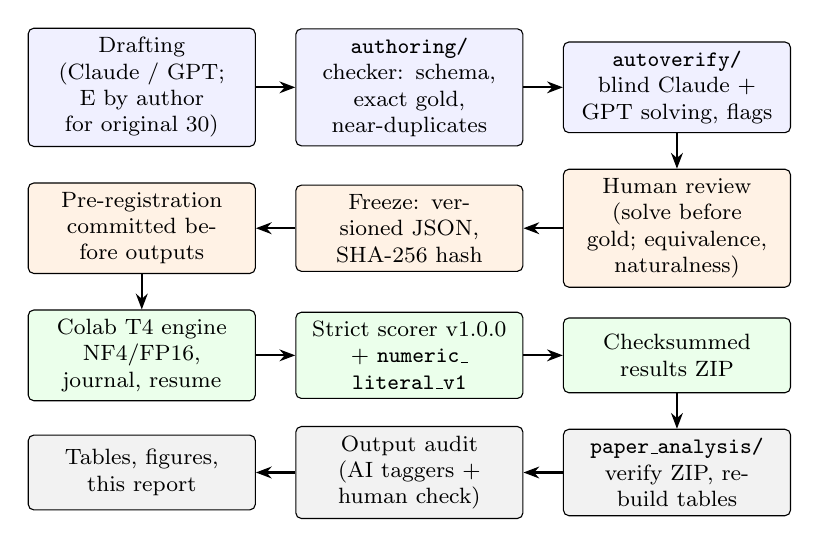
\begin{tikzpicture}[
  node distance=0.45cm and 0.5cm,
  box/.style={draw, rounded corners=2pt, align=center, font=\footnotesize, minimum height=0.95cm, text width=2.65cm, fill=#1},
  box/.default={white},
  arr/.style={-{Stealth[length=2mm]}, thick}]
\node[box=blue!6] (author) {Drafting\\(Claude / GPT; E by author for original 30)};
\node[box=blue!6, right=of author] (check) {\texttt{authoring/}\\checker: schema, exact gold, near-duplicates};
\node[box=blue!6, right=of check] (blind) {\texttt{autoverify/}\\blind Claude + GPT solving, flags};
\node[box=orange!10, below=of blind] (human) {Human review\\(solve before gold; equivalence, naturalness)};
\node[box=orange!10, left=of human] (freeze) {Freeze: versioned JSON, SHA-256 hash};
\node[box=orange!10, left=of freeze] (prereg) {Pre-registration committed before outputs};
\node[box=green!8, below=of prereg] (engine) {Colab T4 engine\\NF4/FP16, journal, resume};
\node[box=green!8, right=of engine] (score) {Strict scorer v1.0.0\\+ \texttt{numeric\_literal\_v1}};
\node[box=green!8, right=of score] (zip) {Checksummed results ZIP};
\node[box=gray!10, below=of zip] (pa) {\texttt{paper\_analysis/}\\verify ZIP, rebuild tables};
\node[box=gray!10, left=of pa] (audit) {Output audit\\(AI taggers + human check)};
\node[box=gray!10, left=of audit] (report) {Tables, figures, this report};
\draw[arr] (author) -- (check);
\draw[arr] (check) -- (blind);
\draw[arr] (blind) -- (human);
\draw[arr] (human) -- (freeze);
\draw[arr] (freeze) -- (prereg);
\draw[arr] (prereg) -- (engine);
\draw[arr] (engine) -- (score);
\draw[arr] (score) -- (zip);
\draw[arr] (zip) -- (pa);
\draw[arr] (pa) -- (audit);
\draw[arr] (audit) -- (report);
\end{tikzpicture}
\caption{Pipeline from drafting to reported tables. Blue: dataset construction; orange: human gate and freeze; green: inference and scoring on Colab; grey: analysis.}
\label{fig:pipeline}
\end{figure}

\section{Evaluation engine and notebooks}

The engine (\texttt{test1\_pilot/hinglish\_pilot/}) handles data validation, the run loop, the Hugging Face backend, reporting and scoring. A builder script packs all of it, with the frozen data, into one self-contained notebook, so a team member just uploads a single \texttt{.ipynb} to Colab and presses \emph{Run all}. A Pilot-B notebook takes about 25--35 minutes on a T4. Research modes refuse the fake test backend, draft data and the wrong split, and every output carries a label saying what kind of evidence it is.

The verified stack is torch 2.11.0+cu130, transformers 4.51.3 and bitsandbytes 0.50.2. Every prompt is tokenized and checked before generation so no question is cut off. CPU offloading, thinking mode, silent cap changes and model substitution are all blocked.

\paragraph{Journal and resume.} Free Colab sessions drop often. Each generation is written to a journal \emph{before} it starts and committed as an atomic JSON file. On resume, the engine refuses to continue if the data, config, code or environment changed, and it skips completed generations even when they are wrong or malformed. A lock file stops two writers sharing one run, and a stale lock is only cleared by an explicit setting. Headline accuracy stays hidden until every output is complete.

\paragraph{Export.} The results ZIP holds manifests, exact inputs and prompts, attempt records, predictions, metrics and a \texttt{checksums.sha256} covering every file. Export uses an allow-list and rejects credential-like patterns.

\section{Scoring details}

The strict scorer looks for exactly one \texttt{FINAL:} line, which must be the last non-blank line, parses an exact rational and checks the unit text against the family's unit, aliases and conversions. Dimensionless answers must carry no suffix. Every failure is stored with an \texttt{invalid\_reason}. The secondary \texttt{numeric\_literal\_v1} never looks at gold while extracting. It accepts an optional \texttt{x =}, a currency \emph{prefix} (\rs, INR, Rs.), a scalar possibly wrapped in \texttt{**}, \texttt{\$} or \verb|\boxed{}|, and an optional word suffix. It has no rule for a currency symbol \emph{after} the number, which matters in Chapter~\ref{ch:results}.

\section{Analysis tools and testing}

\paragraph{\texttt{paper\_analysis/}} turns results ZIPs into tables and figures without extracting or executing anything inside them. It rejects unsafe paths and malformed members, checks every checksum, recomputes accuracy, Wilson intervals and the bootstrap with the engine's formulas, and exits with code 3 on any mismatch. All six cohort runs reproduced their stored metrics exactly.

\paragraph{\texttt{autoverify/}} builds blind solver tasks containing only four whitelisted fields (family ID, rendering ID, form, text), so gold never reaches a solver, and then compares the answers and writes a review sheet with the gold column last. Automated checks never assign ACCEPT. \paragraph{\texttt{authoring/}} checks the schema, evaluates the reference equation in exact fractions and flags near-duplicates (character 5-gram Jaccard $\ge$ 0.5) against the pilot and fixtures.

\paragraph{Tests.} Table~\ref{tab:tests} lists the suites as re-run on 26 October 2026; all 161 tests passed. Beyond unit tests, the notebook ran end-to-end in demo mode, and a real T4 smoke run of Qwen3-4B completed six generations with no infrastructure errors. That smoke run's first 0/6 score exposed a fixture bug and the strict suffix rule on fractions, the first hint of the format issue in Chapter~\ref{ch:dev}.

\begin{table}[t]
\centering\small
\caption{Software test suites (re-run 26 October 2026; all passing).}
\label{tab:tests}
\begin{tabularx}{\linewidth}{@{}lLr@{}}
\toprule
Suite & What it covers & Tests\\
\midrule
\texttt{test1\_pilot/tests} & Engine: scoring, retries, interruption, stale locks, resume, journal corruption, secret detection & 23\\
\texttt{secondary\_analysis/tests} & \texttt{numeric\_literal\_v1} grammar, CMI, notebook freshness & 64\\
\texttt{autoverify/tests} & Task whitelisting, shuffles, flags, review sampling & 23\\
\texttt{t4\_smoke} & Training-protocol validation and completion-only labels & 21\\
\texttt{paper\_analysis/tests} & Safe ZIP reading, checksums, table consistency & 17\\
\texttt{authoring/tests} & Schema, equation exactness, near-duplicates & 10\\
\texttt{pilot/scripts} & Original exact scorer & 3\\
\midrule
Total & & 161\\
\bottomrule
\end{tabularx}
\end{table}

%======================================================================
\chapter{Development Findings and Model Screening}
\label{ch:dev}
%======================================================================

\noindent\textit{Development evidence only.} Everything in this chapter comes from 36 AI-authored, unreviewed fixture prompts (12 families $\times$ E/R/C, \texttt{FMT2}) that are permanently excluded from every cohort, training set and test set. With 12 prompts per form, the rates are rough indications.

Before spending the one-shot cohort runs, we pushed these fixtures through the full pipeline on a T4 to catch protocol problems on data that would never count as evidence.

\section{A format problem in the instruction}

The first instruction (v1) asked for \texttt{FINAL: <number or fraction> <unit when applicable>}. Under it, 10 of 36 Qwen3-4B outputs failed strict scoring, all as \texttt{invalid\_unit} (Table~\ref{tab:fmt2}). In eight of them the model tacked a unit word onto a plain number: \texttt{8 unitless}, \texttt{24 unit.}, \texttt{8 unit (no unit specified, so just the number)}. The phrase ``unit when applicable'' was being taken literally. Since 6 of the 30 original pilot families have dimensionless answers, v1 would have thrown away many correct answers in every form.

\begin{table}[t]
\centering\small
\caption{Qwen3-4B on the 36 excluded FMT2 prompts under prompt v1 and v2 (development evidence; 12 per form).}
\label{tab:fmt2}
\begin{tabular}{@{}llccccc@{}}
\toprule
Prompt & Form & \makecell{Strict\\correct} & \makecell{Numeric\\match} & \makecell{Strict\\invalid} & \makecell{Devanagari\\in output} & \makecell{Median\\output tokens}\\
\midrule
\multirow{3}{*}{v1} & E & 9 & 12 & 3 & 0 & 82\\
 & R & 7 & 10 & 4 & 8 & 107\\
 & C & 9 & 11 & 3 & 0 & 86\\
\midrule
\multirow{3}{*}{v2} & E & 12 & 12 & 0 & 0 & --\\
 & R & 10 & 10 & 0 & 0 & --\\
 & C & 12 & 12 & 0 & 0 & --\\
\bottomrule
\end{tabular}
\end{table}

Decision D020 replaced it with v2: explain in English even if the question is not in English, and after FINAL give an English unit only if the answer has one. The scorer did not change. Under v2 there were 0/36 invalid outputs, plain numbers came back bare (\texttt{FINAL: 8}) and units came back in English (\texttt{330 rupees}). One ambiguous R fixture was also repaired between the runs, so the 10$\to$0 change is a development comparison, not a clean prompt effect. We revised the prompt once, disclosed it, versioned it, and froze it before any cohort output.

\section{Drift into Hindi and two telling errors}

Under v1, 8 of 12 R outputs contained Devanagari although the instruction asked for English; E had none. Under v2 this fell to 0/12. The scorer is not affected, but it showed that instruction following weakens on Romanized-Hindi input, which is why we later audited English compliance.

Under v2, Qwen3-4B's only two errors were both R items. In FMT2-005-R, \emph{bhaag dekar bhinn likho} (``divide, write as a fraction'') was answered as a difference. In FMT2-006-R, \emph{kitna bhinn istemaal hua} (``what fraction was used'') got the remaining count, 20, and Llama-3.2-3B later gave the same 20. \emph{Bhinn} means both ``fraction'' and ``different'', even in Devanagari. Two unreviewed items cannot establish anything, but they are \emph{consistent with} operation-word misreading, and they led us to build the lexicon and the keep/switch balance into Pilot-B.

\section{Seven-model screen}

Decision D028 ran more unchanged models on the same 36 prompts under the frozen v2 prompt and scorer. The rule, fixed before the included models were run, was that a model enters the cohort evaluations only if at most 3/36 outputs are strict-invalid, with no per-model tuning. Table~\ref{tab:screen} shows the outcome.

\begin{table}[t]
\centering\small
\caption{Format screening on the excluded fixtures (prompt v2; strict-invalid of 36; strict correct of 12 per form). Development evidence.}
\label{tab:screen}
\begin{tabularx}{\linewidth}{@{}lccLl@{}}
\toprule
Model & Invalid & E/R/C & Main failure & Decision\\
\midrule
Qwen3-4B & 0 & 12/10/12 & 2 R operation-word misreadings & Primary\\
Qwen3-8B & 0 & 12/12/12 & none & Included (D030)\\
Llama-3.2-3B-Instruct & 2 & 12/9/9 & value errors; 1 truncation, 1 missing FINAL & Included (D032)\\
Qwen3-1.7B & 36 & 0/0/0 & copies the instruction onto the FINAL line & Excluded (D029)\\
Phi-4-mini-instruct & 14 & 6/4/11 & inline FINAL; R repetition to the cap & Excluded (D025)\\
Granite-3.3-2B-instruct & 36 & 0/0/0 & commentary after FINAL & Excluded (D026)\\
Gemma-3-4B-it & -- & -- & CUDA error under FP16, no outputs & Excluded (D031)\\
\bottomrule
\end{tabularx}
\end{table}

The excluded models failed on format, not necessarily on maths. Phi-4-mini and Granite were excluded before the $\le$3/36 rule was formalised; both exceed it. Phi-4-mini wrote the FINAL marker at the end of a paragraph in 7 outputs, and 6 of its 12 R outputs looped until the 1,024-token cap, in four cases repeating the Hindi question 17--40 times; its apparent C~$>$~E ordering (11/12 vs 6/12) is an artifact of that. Granite added comments such as \texttt{FINAL: 24, (units: none)}. Gemma-3-4B loaded but crashed under the frozen FP16 recipe, and fixing that would have meant a model-specific change that D028 does not allow.

Two lessons came out of this. Within Qwen3, instruction following broke before the maths did: 36/36 invalid at 1.7B against 0/36 at 4B and 8B. And one prompt and scorer cannot simply be carried across model families; without this check a multi-model comparison would mostly be measuring formatting.

%======================================================================
\chapter{Phase 1 Results}
\label{ch:results}
%======================================================================

\noindent\textit{Cohort results under pre-registered plans.} Pilot-B (70 families, single reviewer, insertional C) is primary. The original cohort (24 families, clause-based C) is a descriptive replication. The cohorts are never pooled. Each model ran once per cohort and completed every rendering (210/210 and 72/72), and all checksums verified.

\section{Pilot-B accuracy by form}

Table~\ref{tab:pilotb_acc} and Figure~\ref{fig:pilotb} give strict accuracy. R is the lowest-scoring form for every model.

\begin{table}[t]
\centering\small
\caption{Pilot-B strict accuracy (70 families per form): correct count, accuracy (\%) and 95\% Wilson interval, and strict-invalid outputs (truncations in parentheses).}
\label{tab:pilotb_acc}
\setlength{\tabcolsep}{4pt}\footnotesize
\begin{tabular}{@{}lccc@{}}
\toprule
Model & E & R & C\\
\midrule
Qwen3-4B (primary) & 66/70 \enspace 94.3 [86.2, 97.8] & 60/70 \enspace 85.7 [75.7, 92.1] & 66/70 \enspace 94.3 [86.2, 97.8]\\
\quad invalid & 3 & 2 & 1\\
Qwen3-8B & 69/70 \enspace 98.6 [92.3, 99.7] & 64/70 \enspace 91.4 [82.5, 96.0] & 69/70 \enspace 98.6 [92.3, 99.7]\\
\quad invalid & 1 & 1 & 0\\
Llama-3.2-3B & 66/70 \enspace 94.3 [86.2, 97.8] & 40/70 \enspace 57.1 [45.5, 68.1] & 49/70 \enspace 70.0 [58.5, 79.5]\\
\quad invalid & 1 & 6 (5) & 4 (2)\\
\bottomrule
\end{tabular}
\end{table}

\begin{figure}[t]
\centering
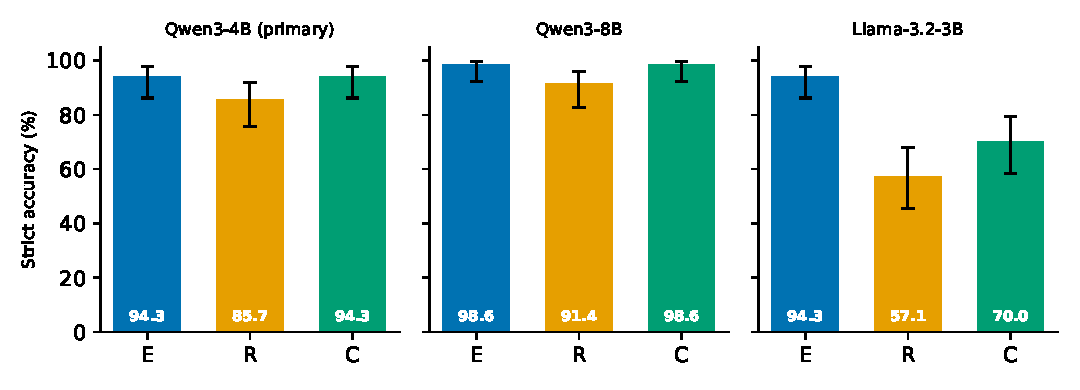
\includegraphics[width=0.92\linewidth]{figures/accuracy_by_form.pdf}
\caption{Pilot-B strict accuracy by form with 95\% Wilson intervals (70 families per bar).}
\label{fig:pilotb}
\end{figure}

\section{Paired differences}

Since all three forms share their families, the right comparison is paired (Table~\ref{tab:pilotb_diff}).

\begin{table}[t]
\centering\small
\caption{Pilot-B paired family differences (pp) with 95\% intervals from 10,000 family-bootstrap resamples (seed 101). In parentheses: families correct only in the first / only in the second form.}
\label{tab:pilotb_diff}
\setlength{\tabcolsep}{2.5pt}\footnotesize
\begin{tabular}{@{}lccc@{}}
\toprule
Model & E$-$R & E$-$C & R$-$C\\
\midrule
Qwen3-4B & $+$8.6 [$-$1.4, $+$18.6] (9/3) & 0.0 [$-$7.1, $+$7.1] (3/3) & $-$8.6 [$-$15.7, $-$1.4] (1/7)\\
Qwen3-8B & $+$7.1 [0.0, $+$14.3] (6/1) & 0.0 [$-$4.3, $+$4.3] (1/1) & $-$7.1 [$-$14.3, 0.0] (1/6)\\
Llama-3.2-3B & $+$37.1 [$+$24.3, $+$50.0] (28/2) & $+$24.3 [$+$11.4, $+$37.1] (21/4) & $-$12.9 [$-$27.1, $+$1.4] (10/19)\\
\bottomrule
\end{tabular}
\end{table}

Four points stand out.
\begin{enumerate}
\item \textbf{R is weakest for all three models}, but by very different amounts: 8.6 and 7.1 points for the two Qwen models (intervals crossing or touching zero) and 37.1 points for Llama (interval well above zero).
\item \textbf{E and C score the same in aggregate for both Qwen models} (E$-$C $=$ 0.0). This is not itemwise identity, since there are 3/3 and 1/1 discordant families, and it is \emph{not an equivalence result}. For Qwen3-4B, C beats R and the R$-$C interval excludes zero.
\item \textbf{For Llama, C sits between E and R}, 24.3 points below E.
\item \textbf{Scale helps but does not close the gap.} Going from Qwen3-4B to 8B lifts R from 85.7\% to 91.4\%, yet the E$-$R gap only moves from 8.6 to 7.1 points.
\end{enumerate}

\section{Operation-word strata}

Table~\ref{tab:strata} splits the results by whether C keeps R's Hindi operation word, switches it to English, or R has none. R accuracy is about the same across strata for every model (Figure~\ref{fig:strata}). The R deficit is \emph{not concentrated} in \emph{bhaag}/\emph{bhinn}-type items, so the misreading idea from the two development errors is not supported at this scale. Many Llama R errors are plain arithmetic slips; in PB017 ($1200 - 3\times265 = 405$) it answered 435.

\begin{table}[t]
\centering\small
\caption{Pilot-B strict accuracy by pre-registered operation-word stratum (descriptive).}
\label{tab:strata}
\begin{tabular}{@{}llcccc@{}}
\toprule
Model & Stratum & Families & E & R & C\\
\midrule
\multirow{3}{*}{Qwen3-4B} & C keeps & 18 & 18 (100\%) & 16 (89\%) & 17 (94\%)\\
 & C switches & 17 & 17 (100\%) & 14 (82\%) & 17 (100\%)\\
 & none & 35 & 31 (89\%) & 30 (86\%) & 32 (91\%)\\
\midrule
\multirow{3}{*}{Qwen3-8B} & C keeps & 18 & 18 (100\%) & 17 (94\%) & 17 (94\%)\\
 & C switches & 17 & 17 (100\%) & 16 (94\%) & 17 (100\%)\\
 & none & 35 & 34 (97\%) & 31 (89\%) & 35 (100\%)\\
\midrule
\multirow{3}{*}{Llama-3.2-3B} & C keeps & 18 & 18 (100\%) & 12 (67\%) & 13 (72\%)\\
 & C switches & 17 & 16 (94\%) & 10 (59\%) & 11 (65\%)\\
 & none & 35 & 32 (91\%) & 18 (51\%) & 25 (71\%)\\
\bottomrule
\end{tabular}
\end{table}

\begin{figure}[t]
\centering
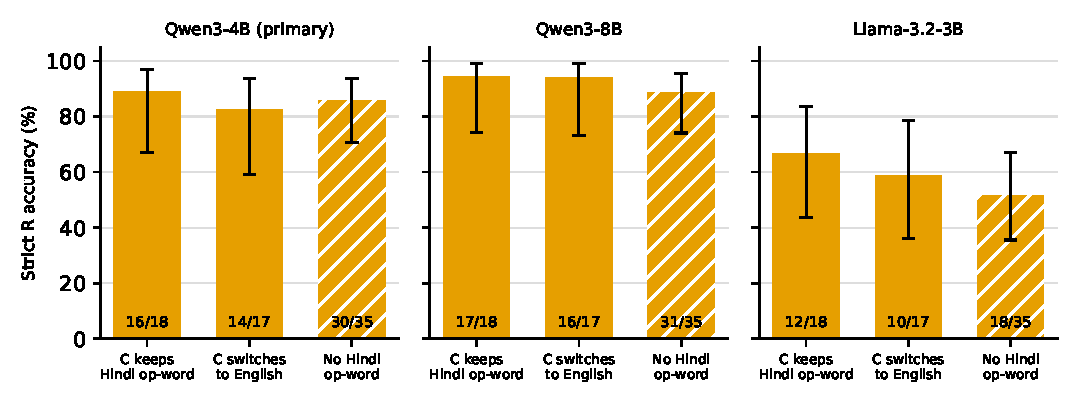
\includegraphics[width=0.92\linewidth]{figures/pilotb_r_by_stratum.pdf}
\caption{Pilot-B strict R accuracy by operation-word stratum with 95\% Wilson intervals.}
\label{fig:strata}
\end{figure}

\section{Format effects that remain}

All six of Qwen3-4B's strict-invalid outputs are \texttt{invalid\_unit}. Three of its four E failures are numerically right answers with English unit phrases outside the alias list (\texttt{11 years old}, \texttt{13 years old}, \texttt{4 bags of cement}), and one C failure is the unlisted spelling \texttt{300 rupye}. Together they cost Qwen3-4B four strict points.

The secondary endpoint has its own gap. Its frozen grammar does not accept a \emph{trailing} rupee symbol (\texttt{FINAL: 1575 \rs}), which the strict scorer accepts. That explains every strict-correct/numeric-fail case (30 for Qwen3-4B, 36 for Qwen3-8B), so for the Qwen models the numeric endpoint falls \emph{below} strict: 72.9/82.9/82.9\% on E/R/C for Qwen3-4B and 84.3/74.3/80.0\% for Qwen3-8B. For Llama the two endpoints agree on all 210 renderings. The gap is in the endpoint's specification, not the models, and we report it as pre-registered without changing it.

\section{Output audit of the primary model}

Claude and GPT each pre-tagged all 210 Qwen3-4B outputs with an error category and an English-compliance tag, blind to each other. They agreed on 206/210 categories (Cohen's $\kappa = 0.94$) and 208/210 compliance tags ($\kappa = 0.96$). A human then checked the 4 disagreements and 20 random agreed rows. Final labels are the human label where checked and the agreed AI label otherwise.

\begin{table}[t]
\centering\small
\caption{Audit category per Qwen3-4B Pilot-B output (70 per form) and English-compliant explanations.}
\label{tab:audit}
\begin{tabular}{@{}lrrr@{}}
\toprule
Category & E & R & C\\
\midrule
no\_error & 66 & 47 & 56\\
format\_only & 3 & 2 & 1\\
language\_drift & 0 & 13 & 10\\
wrong\_relation\_operation & 1 & 4 & 2\\
misread\_quantity & 0 & 2 & 0\\
arithmetic\_slip & 0 & 1 & 1\\
unresolved & 0 & 1 & 0\\
\midrule
English-compliant explanation & 70 & 53 & 59\\
\bottomrule
\end{tabular}
\end{table}

Of Qwen3-4B's 18 strict failures, 6 are format-only. The substantive errors pile up in R: 8, against 1 in E and 3 in C (Table~\ref{tab:audit}). English explanations drop from 70/70 on E to 53/70 on R and 59/70 on C. The \emph{language\_drift} rows are correct answers whose explanation slipped out of English, so instruction following erodes on R and C even when the answer is right. A later post-hoc extension to the two secondary models (three AI taggers, 97 rows human-checked) found the same picture: no format-only R failures for either model, and English R explanations in only 37/70 outputs for Qwen3-8B and 0/70 for Llama.

\section{Original cohort}

All three models completed the 24-family cohort (72/72) with no strict-invalid outputs, and the numeric endpoint agrees with strict throughout. Table~\ref{tab:orig_acc} and Figure~\ref{fig:orig} give the results.

\begin{table}[t]
\centering\small
\caption{Original cohort strict accuracy (24 families per form) with 95\% Wilson intervals, and paired E$-$R difference (pp) with family-bootstrap interval.}
\label{tab:orig_acc}
\setlength{\tabcolsep}{3pt}\footnotesize
\begin{tabular}{@{}lcccc@{}}
\toprule
Model & E & R & C & E$-$R\\
\midrule
Qwen3-4B & 24/24 \enspace 100.0 & 22/24 \enspace 91.7 [74.2, 97.7] & 24/24 \enspace 100.0 & $+$8.3 [0.0, $+$20.8]\\
Qwen3-8B & 24/24 \enspace 100.0 & 23/24 \enspace 95.8 [79.8, 99.3] & 24/24 \enspace 100.0 & $+$4.2 [0.0, $+$12.5]\\
Llama-3.2-3B & 21/24 \enspace 87.5 & 15/24 \enspace 62.5 [42.7, 78.8] & 22/24 \enspace 91.7 & $+$25.0 [$+$4.2, $+$45.8]\\
\bottomrule
\end{tabular}
\end{table}

\begin{figure}[t]
\centering
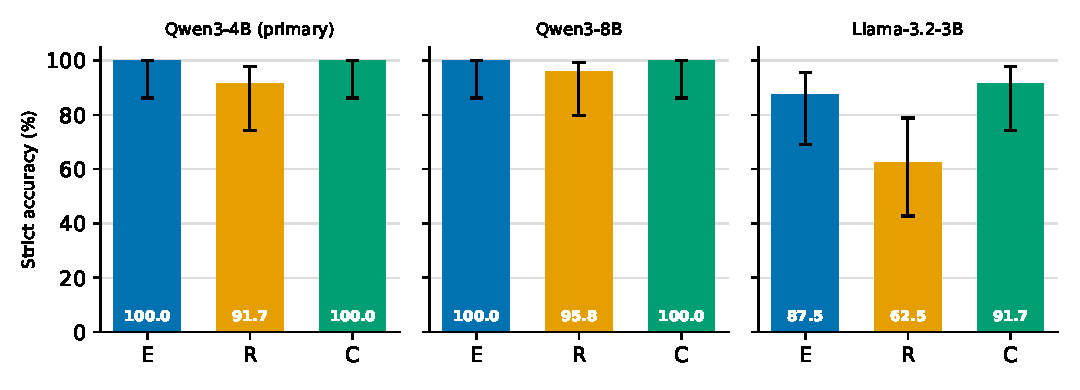
\includegraphics[width=0.92\linewidth]{figures/original_cohort_accuracy.pdf}
\caption{Original cohort strict accuracy by form with 95\% Wilson intervals (24 families per bar).}
\label{fig:orig}
\end{figure}

The direction holds: R is lowest for every model in both cohorts. Qwen is near ceiling here (E $=$ C $=$ 100\%). Qwen3-4B's two R errors include PIL001-R, where \emph{Riya se 5 kam} (``5 fewer than Riya'') was treated as addition, a genuine one-off operation-word misreading. Llama's C, unlike in Pilot-B, sits at E's level here (91.7\% vs 87.5\%), so where C falls relative to E depends on both model and cohort.

\section{A note on token length (post hoc)}

\noindent\textit{Post-hoc and exploratory, written after all outputs were seen; no multiplicity correction, no causal claim.}

With the pinned Qwen3 tokenizer, R questions are clearly longer than E at about the same word count: a median of $+$15 tokens per family (ratio 1.42; R longer in 70/70) in Pilot-B and $+$22.5 (ratio 1.61) in the original cohort. R words split into more pieces (2.00 vs 1.45 tokens per word in Pilot-B). C is longer too, by about 8 tokens, yet Qwen's C accuracy equals its E accuracy. For the Qwen models, R-wrong families were not longer than R-correct ones (median R$-$E 15 vs 14 tokens for Qwen3-4B). For Llama in Pilot-B there was a weak association (16.5 vs 13.5 tokens, $p = 0.073$) that did not appear in the original cohort. We therefore treat length as at most a minor correlate, not the cause of the R gap.

\section{What Phase 1 tells us}

The hard case was Romanized Hindi, not code-mixing. Hinglish was never the lowest form, and for both Qwen models it matched English in observed aggregate accuracy. One plausible reason is that insertional Hinglish keeps English content words like \emph{ratio}, \emph{add} and \emph{total}, which may anchor the model. We should not overstate it: E $=$ C here is equal observed proportions, not equivalence, and for Llama in Pilot-B C is 24.3 points below E. Since all three forms are in Latin script, we also cannot separate a romanization penalty from a Hindi-vocabulary or register effect.

The size of the R gap varies four- to fivefold between models, while Llama matches Qwen3-4B on English (94.3\% each). A result on one model family is a weak guide to another. Our direction agrees with CodeMixTax~\citep{sthanika-2026-codemix}, whose gaps are larger; since models, items and protocols all differ, the magnitudes cannot be compared directly. The scoring findings echo \citet{peter-etal-2026-mind}: one phrase in an instruction created form-dependent failures, and even a carefully specified extractor had a blind spot.

%======================================================================
\chapter{Phase 2: Fine-Tuning Study}
\label{ch:phase2}
%======================================================================

\noindent\textit{Completed pre-registered study.} Strict-accuracy $\Delta_C$ is the only confirmatory estimand. Everything else is descriptive.

\section{Design}

Phase~2 asks whether training on Hinglish rather than Romanized Hindi improves accuracy on Hinglish questions. The essential comparison (D001) is three arms with matched content, matched exposure and identical English solution targets:
\begin{itemize}
\item \textbf{E+E}: each TRAIN family gives the English solution twice, both times from the E question;
\item \textbf{E+R}: once from the E question and once from the R question;
\item \textbf{E+C}: once from the E question and once from the C question.
\end{itemize}
TRAIN has 160 families, so each arm sees 320 examples. DEV (40 families) is used only for sanity checks, never to choose anything. FINAL\_TEST (100 families) is evaluated once, after all adapters are frozen. The labels mask the prompt and supervise only the English solution, and we assert that the target tokens are identical across E, R and C before training starts.

\paragraph{Feasibility.} Before fixing anything we ran a smoke test on a Colab T4 (D041--D042). All three arms ran at about 20~s per update (19.8/20.4/20.6~s), well under the 56~s threshold set in advance by D021, with peak memory around 5~GB and exact checkpoint reload. The smoke run also showed that 16 families were memorised within about 12 passes, so the provisional 256-update plan risked the same memorisation regime.

\paragraph{Recipe (D043).} Qwen3-4B with QLoRA: NF4 double-quantized base, FP16 compute, LoRA rank 16 and alpha 32 on all seven linear projections, 16 examples per update, \textbf{3 passes $=$ 60 updates}, AdamW at $10^{-4}$ with six warm-up updates and cosine decay to $10^{-5}$. Seeds 11, 22 and 33 are paired: within a seed, family order and initial adapter are identical across the three arms. Only the checkpoint after update 60 is evaluated. This schedule was a feasibility choice, not a tuned optimum.

\section{Estimand and decision rule}

Let $y(i,s,a,l)$ be strict correctness for family $i$, seed $s$, arm $a$ and test form $l$. The confirmatory contrast is
\[
 \Delta_C=\frac{1}{100}\sum_{i=1}^{100}\frac{1}{3}\sum_{s\in\{11,22,33\}}\bigl[y(i,s,EC,C)-y(i,s,ER,C)\bigr].
\]
We use a paired family bootstrap with 10,000 resamples. The labels were fixed before training (D040, frozen in the pre-registration D044): \emph{Support} if the lower bound is above 0; \emph{Useful support} if above $+5$; \emph{Informative null} if the interval contains 0 and its upper bound is below $+5$; \emph{Harm} if the upper bound is below 0; otherwise \emph{Inconclusive}. Identical family contrasts or a zero-width interval override these labels as inconclusive (degenerate interval). A planning simulation had shown that 100 families give about $\pm$2--5 points of precision ($\pm$3--4 in the central cases), so a small gain would be hard to detect. English retention used a $-$2-point margin.

\section{Execution}

All nine training runs were valid at the first attempt: 60/60 updates each, no scaler skips and no resumption. On 7 November Colab's default image moved to a newer torch; the notebook refused to start, and later runs used an older runtime with the registered torch 2.11.0+cu130, so the stack never changed. The adapters were frozen on 8 November (D051). The unchanged model scored 33/19/24 of 40 on DEV, so the pre-declared ceiling flag (C $\ge$ 38/40) did not fire (D049). Two evaluation sessions were interrupted and resumed from their journals without regenerating any answer; all 3,000 required generations resolved. The registered analysis ran once on 10 November (D052).

Two disclosures matter. FINAL\_TEST had been seen by its drafting and checking models and its reviewer during construction. And on 3 November some unattended CPU tests parsed its file, which went beyond the hash-only access rule; this is disclosed in Amendments~2--3, and the data, design and thresholds did not change.

\section{Confirmatory result}

\[
 \Delta_C=-4.33\ \mathrm{pp},\qquad 95\%\ \mathrm{interval}\ [-8.00,-0.67]\ \mathrm{pp}.
\]
The upper bound is below zero, so the registered label is \textbf{Harm}. All three seeds are negative ($-3.00$, $-1.00$ and $-9.00$ points). The companion Wald interval is $[-8.01,-0.66]$; the conservative Hoeffding interval is much wider, $[-31.50, +22.83]$. An independent re-computation from the raw predictions agreed exactly. Under this recipe, E+C scored 42.7\% on C against 47.0\% for E+R. This is a statement about E+C relative to E+R under one frozen recipe, not a claim that Hinglish training is harmful in general.

\begin{table}[t]
\centering\small
\caption{Strict accuracy (\%) on FINAL\_TEST for every checkpoint (100 families per cell).}
\label{tab:phase2-acc}
\begin{tabular}{@{}lccc@{\hspace{1.2cm}}lccc@{}}
\toprule
Checkpoint & E & R & C & Checkpoint & E & R & C\\
\midrule
EE:11 & 62 & 41 & 44 & ER:33 & 61 & 37 & 50\\
EE:22 & 63 & 41 & 41 & EC:11 & 64 & 43 & 41\\
EE:33 & 59 & 39 & 44 & EC:22 & 58 & 41 & 46\\
ER:11 & 61 & 42 & 44 & EC:33 & 54 & 40 & 41\\
ER:22 & 56 & 35 & 47 & unchanged & 85 & 63 & 66\\
\bottomrule
\end{tabular}
\end{table}

\section{Secondary results}

\paragraph{English loss.} The bigger practical finding is in Table~\ref{tab:phase2-acc}: every trained checkpoint is below the unchanged model in every form. On English the strict losses against the unchanged model are $-26.33$ points for E+C $[-34.33,-19.00]$, $-25.67$ for E+R and $-23.67$ for E+E, all flagged as loss beyond the margin. E+E loses too, so swapping English for Hinglish is not what causes it. Trained answers were also far shorter: a median of 42 tokens against 113 for the unchanged model. Back on DEV (D050) we had noticed the first E+C adapter writing shorter answers (mean 43 vs 121 tokens), and the shared English reference solutions were terse. That pattern is \emph{consistent with} the short targets being the problem, but the design cannot prove it.

\paragraph{R transfer and specificity.} E+R minus E+E on R was $-2.33$ $[-9.33,+4.33]$ and E+C minus E+R on R was $+3.33$ $[-2.00,+8.67]$; both intervals include zero. The numeric endpoints agree in direction with strict on C ($-5.67$ $[-11.00,-0.67]$).

\paragraph{Operation-word strata.} $\Delta_C$ was negative in every stratum: $-1.3$ (keep, 25 families), $-6.7$ (none, 50) and $-2.7$ (switch, 25). These are descriptive counts.

\section{Failure audit}

To check that the Harm result is not just a formatting artifact, we audited every strict-incorrect C output from E+R and E+C: 159 and 172 failures, 331 in all. GPT and Claude tagged them blind to each other (category agreement 301/331, $\kappa = 0.869$), and two bilingual team members, Ayush Kumar Singh and Divyanshu Mishra, then labelled all 331, so every final label is a human label.

\begin{table}[t]
\centering\small
\caption{Final C-failure audit. Substantive is the subtotal of the four mathematical-error rows.}
\label{tab:phase2-final-audit}
\begin{tabular}{@{}lrrr@{}}
\toprule
Classification & E+R & E+C & Total\\
\midrule
Format-only & 46 & 40 & 86\\
Misread quantity & 33 & 36 & 69\\
Wrong relation/operation & 65 & 77 & 142\\
Arithmetic slip & 7 & 11 & 18\\
Unit error & 8 & 8 & 16\\
\midrule
Substantive subtotal & 113 & 132 & 245\\
All failures & 159 & 172 & 331\\
\bottomrule
\end{tabular}
\end{table}

E+C has \emph{fewer} format-only failures than E+R but \emph{more} substantive ones (132 vs 113), mostly wrong relations or operations (Table~\ref{tab:phase2-final-audit}). The E+C deficit is real mathematical error, not a scoring quirk. The audit cannot tell us the training mechanism behind it.

\section{What Phase 2 tells us}

Under this recipe, giving the model Hinglish questions during training did not help it on Hinglish test questions; it did slightly worse than training on Romanized Hindi. The larger effect was that all three arms lost a quarter of their English accuracy and started writing much shorter answers. The comparison was therefore between similarly degraded models. That is what motivated Phase~3.

%======================================================================
\chapter{Phase 3: Training on the Model's Own Solutions}
\label{ch:phase3}
%======================================================================

\noindent\textit{Work in progress.} Training is complete and the adapters are frozen. The single test evaluation has not been run, so no Phase-3 result is reported here.

\section{Question and design}

In Phase~2 every arm lost about 24--26 points of English accuracy while its answers shrank from a median of 113 to 42 tokens. Phase~3 asks whether the Phase-2 conclusion changes when the training targets are written in the model's own style: does E+C beat E+R on Hinglish questions when the targets are the unchanged Qwen3-4B's own correct English answers (\emph{self-distillation})?

Everything except the targets is kept from Phase~2: the same three arms with identical English targets across forms, the same QLoRA recipe and 60 updates, paired seeds 11/22/33, the same strict scorer, the same estimand $\Delta_C$ and the same decision labels. The unchanged model was run once on the English version of each of the 160 TRAIN families. An answer became a target only if it was strictly correct, complete, fully English and short enough for every form, and the plan said in advance that the study would halt if fewer than 120 families qualified. The 100 FINAL\_TEST families are reused, which we disclose as a limitation, because Phase~3 was designed after seeing Phase~2.

\section{Status}

\begin{itemize}
\item \textbf{Pre-registration} adopted before any Phase-3 output (D053).
\item \textbf{Targets:} 160 answers generated on a T4; 158 qualified (two were wrong), none needed language review, and the median target is 106 tokens (D054--D055).
\item \textbf{Implementation} passed an independent adversarial review; one blocking defect was fixed before the freeze (D056).
\item \textbf{Training:} all nine runs (three arms $\times$ seeds 11/22/33) completed at the first attempt between 21 and 26 November, each with 60/60 updates, no skipped updates and no resumption. Paired seeds shared the same data order and initial adapter, as planned.
\item \textbf{Incident:} one Colab session ended during a run's DEV sanity check. After the registered recovery, the evaluation validator was amended to accept the engine's documented record of the interrupted generation; the training code did not change (D058).
\item \textbf{Freeze:} adapters frozen on 26 November ($S=3$, confirmatory) and the sealed FINAL\_TEST package built.
\item \textbf{Next:} the single test evaluation (nine adapters, 2,700 generations).
\end{itemize}
The DEV numbers from these runs are sanity checks only and are not reported as results.

\section{How we will read the outcome}

If E+C now beats E+R (\emph{Support}), the Phase-2 harm was tied to the short-target recipe. If the result is again Harm or an informative null, Hinglish exposure does not help even when the model keeps its own style. Either way, comparing each arm with its Phase-2 counterpart will show, descriptively, how much of the English loss came from the style of the targets.

%======================================================================
\chapter{Limitations, Ethics and AI Use}
\label{ch:limits}
%======================================================================

\section{Limitations}

\paragraph{Small samples.} With 70 and 24 families the intervals are wide, and the operation-word strata (17--35 families) are descriptive only. The original cohort is near ceiling for Qwen, and its plan was written after Pilot-B results were known.

\paragraph{Few reviewers.} Pilot-B, FINAL\_TEST and the lexicon were each reviewed by one bilingual team member, and TRAIN/DEV by a 45-family sample. Naturalness reflects very few speakers. A second-annotator sample is planned (D027).

\paragraph{AI-drafted items.} Most renderings were drafted by an LLM and may share its style. Claude both drafted and blind-solved Pilot-B.

\paragraph{Review integrity.} The original pilot's review hit several problems: non-independent early rounds, byte-identical re-reviews and an AI-prefill marker in one reviewer's file. Each was handled by \emph{excluding} the affected evidence before any model output, never by patching it afterwards.

\paragraph{Design limits.} The two cohorts use different C definitions. There is no Devanagari arm, so the E$-$R gap mixes script, language, register and spelling. Two Qwen sizes and one Llama model do not cross scale with family, and the screen left out four of seven models. All runs use NF4, FP16 and greedy decoding on a T4; no cross-hardware bitwise reproducibility is claimed. Pretraining contamination cannot be audited.

\paragraph{Scoring.} Strict scoring still penalises some correct answers (\texttt{11 years old}, \emph{rupye}), and the secondary endpoint has the trailing-\rs\ gap. Both are reported, not corrected. The prompt was revised once after seeing 12 unreviewed fixtures, and this is disclosed.

\paragraph{Training study.} The Phase-2 result covers one model, one frozen recipe and 100 test families. The bootstrap interval does not include seed-to-seed training variation. Because every arm lost about a quarter of its English accuracy, the comparison is between similarly degraded models.

\section{Ethics}

Reviewers received a consent note covering the task, data use and release, and all consented to release under CC BY 4.0. They appear only under pseudonyms (R01, R02, A01), and the adjudicator declined credit. The human checks of the output audits were done by team members Ayush Kumar Singh and Divyanshu Mishra. The items are invented everyday problems with invented first names. Data are released under CC BY 4.0 and code under the MIT licence (D034).

\section{AI-assistance disclosure}
\label{sec:aidisclosure}

AI assistants were used heavily in this project. Specifically:
\begin{enumerate}
\item \textbf{Drafting items.} Renderings were drafted by an LLM: Claude for Pilot-B and TRAIN, GPT for FINAL\_TEST and DEV. For the original pilot the author wrote the English statements and GPT (via Codex) translated R and C. Every family was then checked against code-computed gold and reviewed by humans, and the AI-drafted sets were also verified blind by two LLM solvers (with the FT057-C exception noted in Section~3.5).
\item \textbf{Review.} Humans made every acceptance decision. Some lexicon entries and text edits were drafted by AI before reviewers confirmed them. One reviewer's AI-prefilled, unverified judgments in the original cohort were excluded.
\item \textbf{Audits.} The Pilot-B audit used Claude and GPT as pre-taggers with a human check. The post-hoc extension used Claude Opus, GPT and Claude Sonnet with a 97-row human check. The Phase-2 failure audit used GPT and Claude Opus, blind to each other, with a human check of all 331 outputs.
\item \textbf{Writing, code and decisions.} AI assistants helped write the evaluation and analysis code, the research notes, the paper draft and this report. Under the team's explicit delegation (D017) they also recorded protocol decisions in the decision log, each labelled as an AI decision under delegation. The Phase-2 protocol draft, power simulation (D040) and smoke-test code (D041) were written by a Claude Opus subagent while GPT access had lapsed; the smoke-test code has no independent GPT cross-check yet. In Phase~2 Claude coordinated the runs and analysis, GPT (Astra) drafted the Phase-2 chapter of the full report, and GPT (Sol) independently re-computed the confirmatory result, with exact agreement. The team reviewed this work and takes responsibility for it.
\end{enumerate}
Systems used: Claude Opus 5.5 and Claude Sonnet (Anthropic); GPT-6 Astra and GPT-6.1 Sol (OpenAI, via the Codex CLI).

%======================================================================
\chapter{Conclusion and Future Work}
\label{ch:conclusion}
%======================================================================

\section{Conclusion}

With the maths held fixed, three small open models were least accurate on Romanized Hindi in two separately reviewed, pre-registered cohorts. The size of the drop depended strongly on the model: about 7--9 points for Qwen and 25--37 for Llama. Both Qwen models had the same observed aggregate accuracy on English and Hinglish. The R errors did not cluster around Hindi operation words, and models drifted away from English explanations on non-English input. On the methods side, we learned that a single phrase in an answer-format instruction can produce form-dependent scoring failures, so formats and scorers must be checked on excluded data before any language comparison is run.

In Phase~2, training on Hinglish did not help with Hinglish. E+C scored 42.7\% on C against 47.0\% for E+R ($\Delta_C = -4.33$ points $[-8.00, -0.67]$, Harm), with all three seeds negative, an exact independent re-computation and a human-checked audit showing the extra failures are substantive. Every trained arm also fell well below the unchanged model and wrote much shorter answers. Phase~3, which trains on the model's own solutions, has finished training and is ready for its single test evaluation.

\section{Timeline}

\begin{table}[H]
\centering\small
\caption{Status and plan (as of 26 November 2026).}
\label{tab:timeline}
\begin{tabularx}{\linewidth}{@{}lL@{}}
\toprule
Period & Milestone\\
\midrule
Oct 2026 (done) & Original-cohort runs; SRW mentorship submission \#12 (26 Oct); Pilot-B audit; Phase-2 protocol and power simulation; T4 smoke test, GO.\\
Nov 2026 (done) & Phase 2: schedule fixed, pre-registration frozen and amended, nine valid runs, single FINAL\_TEST evaluation (Harm, 10 Nov), audits. Phase 3: pre-registration, targets, implementation freeze, nine valid runs (21--26 Nov), adapter freeze (26 Nov).\\
Dec 2026 -- Jan 2027 & Phase-3 test evaluation, analysis, verification and failure audit. SRW mentor feedback (5 Dec), final submission (15 Dec), notification (5 Jan).\\
Feb -- Mar 2027 & Training paper (Phases 2 and 3) for ARR; second-annotator sample; extensions.\\
Apr -- May 2027 & Thesis draft and final submission.\\
\bottomrule
\end{tabularx}
\end{table}

\section{Publication plan}

Under D023 the Phase-1 findings target the EACL 2027 Student Research Workshop as a 4-page short paper. It went to the SRW pre-submission mentorship on 26 October 2026 (submission \#12, D039); mentor feedback is due on 5 December and the final paper by 15 December 2026. The training study targets the ARR May 2027 cycle, whose date is not yet confirmed. Co-authorship with the faculty guide will be discussed with the guide.

\section{Future work}

\begin{itemize}
\item A fresh, never-used test set, so the training comparison no longer relies on a reused one.
\item A reviewed Devanagari arm to separate script from language, and independently written spelling variants of R.
\item A second independent language reviewer for every cohort, and a full human audit of outputs.
\item More model families at matched sizes.
\item Content-fixed interventions (word swaps, length padding) to test whether token length plays any causal role.
\end{itemize}

%======================================================================
\cleardoublepage
\phantomsection
\addcontentsline{toc}{chapter}{References}
\renewcommand{\bibname}{References}
{\setstretch{1.1}
\bibliographystyle{unsrtnat}
\bibliography{references}}

%======================================================================
\appendix

\chapter{Frozen Prompt and Hashes}
\label{app:prompt}

\section*{Frozen prompt}

The system message used for every form and every model (\texttt{test1-english-final-v2}, D020):

\begin{quote}\small\ttfamily\raggedright
Solve the problem. Give a short explanation in English, even if the question is not in English. End with exactly one line: FINAL: <number or fraction>, followed by its unit in English only if the answer has a unit; write nothing after a pure number or fraction.
\end{quote}

The user message is the question text alone. The superseded v1 asked for \texttt{FINAL: <number or fraction> <unit when applicable>}; the phrase ``unit when applicable'' caused unit words on dimensionless answers (Chapter~\ref{ch:dev}).

\section*{Dataset and model hashes}
\label{app:hashes}

All hashes are SHA-256. Run ZIP hashes and the full reproduction steps are kept in the repository and in the full project report.

\begin{table}[h]
\centering\footnotesize\singlespacing
\caption{Frozen dataset files and pinned model revisions.}
\label{tab:hashes}
\begin{tabularx}{\linewidth}{@{}lrL@{}}
\toprule
File & Families & SHA-256\\
\midrule
\texttt{pilot\_b/pilot\_b\_families.v2.json} & 70 & \hash{e632e5fcc6b050e93d85920d7938fbb229936fa1474095d6c4c4a6517fcf3478}\\
\texttt{phase2/final\_test.v3.json} & 100 & \hash{da89dd9a626e438dffca39e3a74c4c8abac6bb57501495723b87e6ee143f3d46}\\
\texttt{phase2/train\_A.v2.json} & 80 & \hash{b9656a8c41af2a795bce9c131efc6a5efc652df78368d14fb7720fd985883666}\\
\texttt{phase2/train\_B.v2.json} & 80 & \hash{c975fe12459df6160effc5aeb0087f94666ba0b49778c3d827a67bb923ff35bd}\\
\texttt{phase2/dev.v2.json} & 40 & \hash{e741c1652f5b3dcaebc78d9dd9d7c31fdf4417306fbb2f0862149f27f858f28b}\\
\texttt{pilot\_original/cohort\_dataset.json} & 24 & \hash{5c3e8746f0629d1908902658bda2c280aeb388c55e741fb8e612bc49b5d43103}\\
\midrule
Model & & Pinned revision\\
\midrule
\texttt{Qwen/Qwen3-4B} & & \texttt{1cfa9a7208912126459214e8b04321603b3df60c}\\
\texttt{Qwen/Qwen3-8B} & & \texttt{b968826d9c46dd6066d109eabc6255188de91218}\\
\texttt{meta-llama/Llama-3.2-3B-Instruct} & & \texttt{0cb88a4f764b7a12671c53f0838cd831a0843b95}\\
\bottomrule
\end{tabularx}
\end{table}

\end{document}
